% !TEX encoding = UTF-8
%Koma article
\documentclass[fontsize=12pt,paper=letter,twoside]{scrartcl}
\usepackage{float}
\usepackage{listings}

%Standard Pre-amble
\usepackage[top=4cm,bottom=4cm,left=3cm,right=3cm,asymmetric]{geometry}
%\geometry{landscape}                % Activate for for rotated page geometry
%\usepackage[parfill]{parskip}    % Begin paragraphs with an empty line rather than an indent
\usepackage[table,xcdraw]{xcolor}
\usepackage{graphicx}

\usepackage{amsmath}
\usepackage{amssymb}
\usepackage{epstopdf}
\DeclareGraphicsRule{.tif}{png}{.png}{`convert #1 `dirname #1`/`basename #1 .tif`.png}
% Listings needs package courier
\usepackage{listings} % Needs 
\usepackage{courier}

\usepackage[framemethod=TikZ]{mdframed}
\usepackage{url}

\usepackage{sty/bsymb} %% Event-B symbols
\usepackage{sty/eventB} %% REQ and ENV
\usepackage{sty/calculation}

%Maths
\usepackage{amssymb,amsmath}
\def\Fl{\mathbb{F}}
\def\Rl{\mathbb{R}}
\def\Nl{\mathbb{N}}
\def\Bl{\mathbb{B}}
\def\St{\mathbb{S}}
\newcommand{\ovr}{\upharpoonright}
\newcommand{\var}[1]{\textit{#1}}
%Useful definitions
\newcommand{\mv}[1]{\textit{m\_#1}}
\newcommand{\cv}[1]{\textit{c\_#1}}
\newcommand{\degree}[1]{^{\circ}\mathrm{#1}}
%\newcommand{\comment}[1]{{\footnotesize \quad\texttt{--}\textrm{#1}}}
\newcommand{\im}[1]{i\texttt{-\!#1}}

\usepackage[headsepline]{scrpage2}
\pagestyle{scrheadings}
\ihead[]{\small EECS4312 Report1}
\ohead[]{\small \thepage}
\cfoot[]{}
\ofoot[]{}


%%%%PVS environment%%%%%%%%%%%%%%%%%%%
\lstnewenvironment{pvs}[1][]
    {\lstset{#1,captionpos=b,language=pvs,
    mathescape=true,
    basicstyle=\small\ttfamily,
    numbers=none,
    frame=single,
    % numberstyle=\tiny\color{gray},
    % backgroundcolor=\color{lightgray},
    firstnumber=auto
    }}
    {}
 %%%%%%%%%%%%%%%%%%%%%%%%%%%%%%%%
 
%%%%Verbatim environment%%%%%%%%%%%%%%%%%%%
\lstnewenvironment{code}[1][]
    {\lstset{#1,captionpos=b,
    mathescape=true,
    basicstyle=\small\ttfamily,
    numbers=none,
    frame=single,
    % numberstyle=\tiny\color{gray},
    % backgroundcolor=\color{lightgray},
    firstnumber=auto
    }}
    {}

% \newenvironment{boxed}[1]
%    {\begin{center}
%    #1\\[1ex]
%    \begin{tabular}{|p{0.9\textwidth}|}
%    \hline\\
%    }
%    { 
%    \\\\\hline
%    \end{tabular} 
%    \end{center}
%    }
 %%%%%%%%%%%%%%%%%%%%%%%%%%%%%%%%
 
 %Text in a box
\newenvironment{textbox}
    {\begin{center}
    \begin{tabular}{|p{0.9\textwidth}|}
    \hline\\
    }
    { 
    \\\\\hline
    \end{tabular} 
    \end{center}
    }

\usepackage{hyperref}

%Highlight \hl{}
\usepackage{soul}

\usepackage{enumitem}
\newlist{mylist}{itemize}{1}
\setlist[mylist]{label=\textbullet,leftmargin=1cm,nosep}

\usepackage{multirow}

% Reduce space between figure and caption
%\usepackage{caption}
%\captionsetup[table]{font=small,skip=0pt}     %% Adjust here
%or equivalently 
\usepackage[font=small,skip=4pt]{caption}
%Useful definitions
%\newcommand{\mv}[1]{\textit{m\_#1}}
%\newcommand{\cv}[1]{\textit{c\_#1}}
%\newcommand{\degree}[1]{^{\circ}\mathrm{#1}}
%\newcommand{\comment}[1]{{\footnotesize \quad\texttt{--}\textrm{#1}}}

% Set the header
\ihead[]{\small Gradapps}


%%%%%%%%%%%%Enter your names here%%%%%%%%
\author{\textbf{Edward Vaisman}
\and \textbf{Sadman Sakib Hasan}
}
%%%%%%%%%%%%%%%%%%%%%%%%%%%%%%%%

\date{\today} % Display a given date or no date

\begin{document}
\title{Grad Apps 2.0 \\ Admission Committee Member User Manual}
\maketitle

\newpage

%%%%%%%%%%%%%%%%%%%%%%%%%%%%%%%
\tableofcontents

\newpage


%%%%Rest of your document goes here%%%%%%%%%%%%%%%%%%%

\clearpage
\section{Logging In}

To access the gradapps portal you'll first need to be authenticated into the system. To begin simply click on the ``Sign In" button on the welcome page.

\begin{figure}[!htb]
\begin{center}

\includegraphics[width=.99\textwidth]{images/welcome.png}
\end{center}
\caption{Welcome Page}
\label{fig:welcome}
\end{figure}

\bigskip

You will then be redirected to the login page. Input your username, password and click on the ``Login" button. If you are successfully authenticated you will be redirected to the role selection page.

\begin{figure}[!htb]
\begin{center}
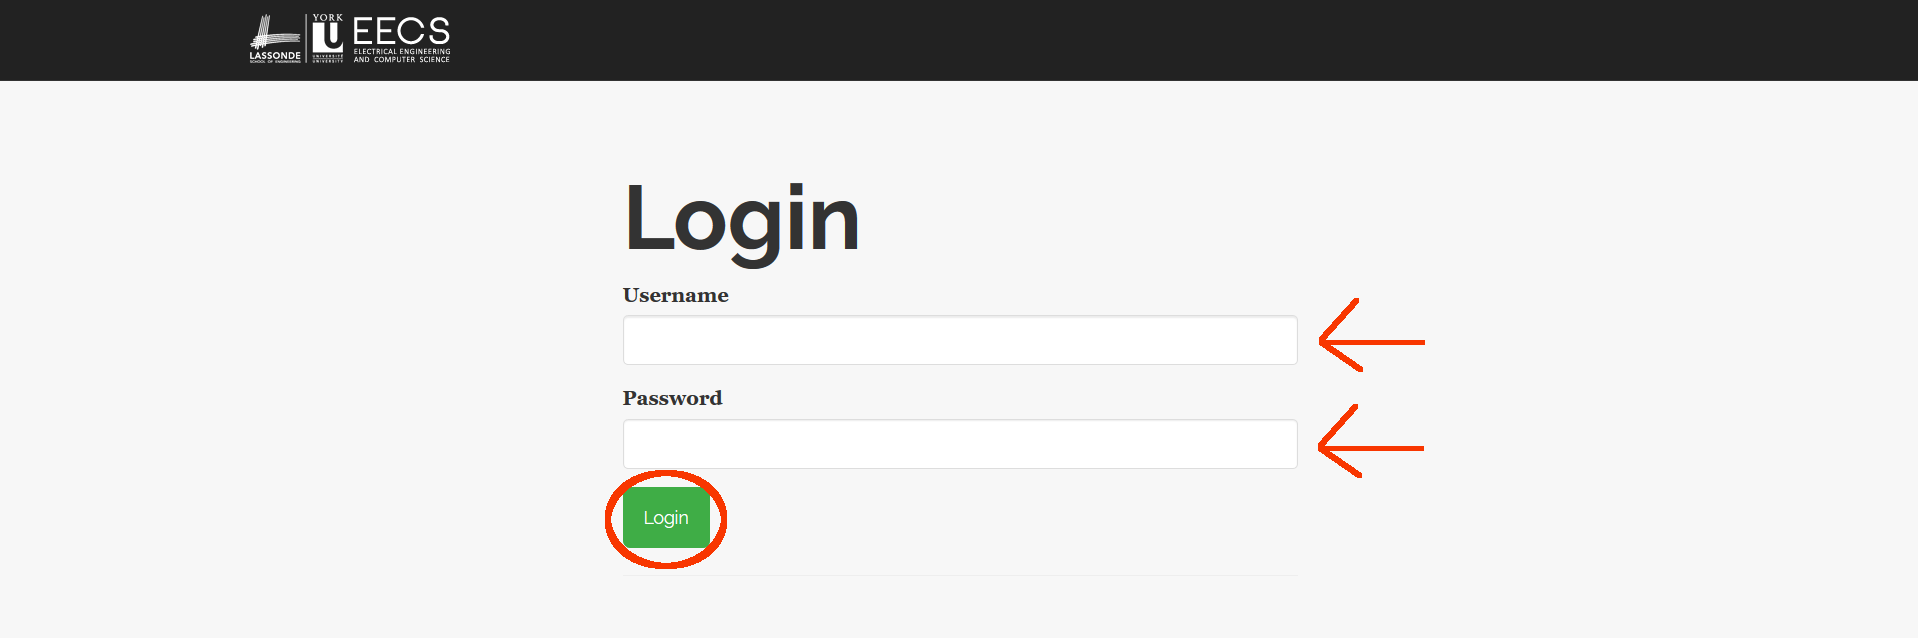
\includegraphics[width=.99\textwidth]{images/login.png}
\end{center}
\caption{Login Page}
\label{fig:login}
\end{figure}
\noindent \textbf{Note:} If the credentials you have provided are invalid you will be greeted with an error message.

\clearpage

\section{Selecting a Role}
The subsections below describe the methods for selecting the a role.

\subsection{Role Selection Page}
From the role selection page click on the ``Continue as Committee Member" button to be redirected to the committee member portal.

\begin{figure}[!htb]
\begin{center}
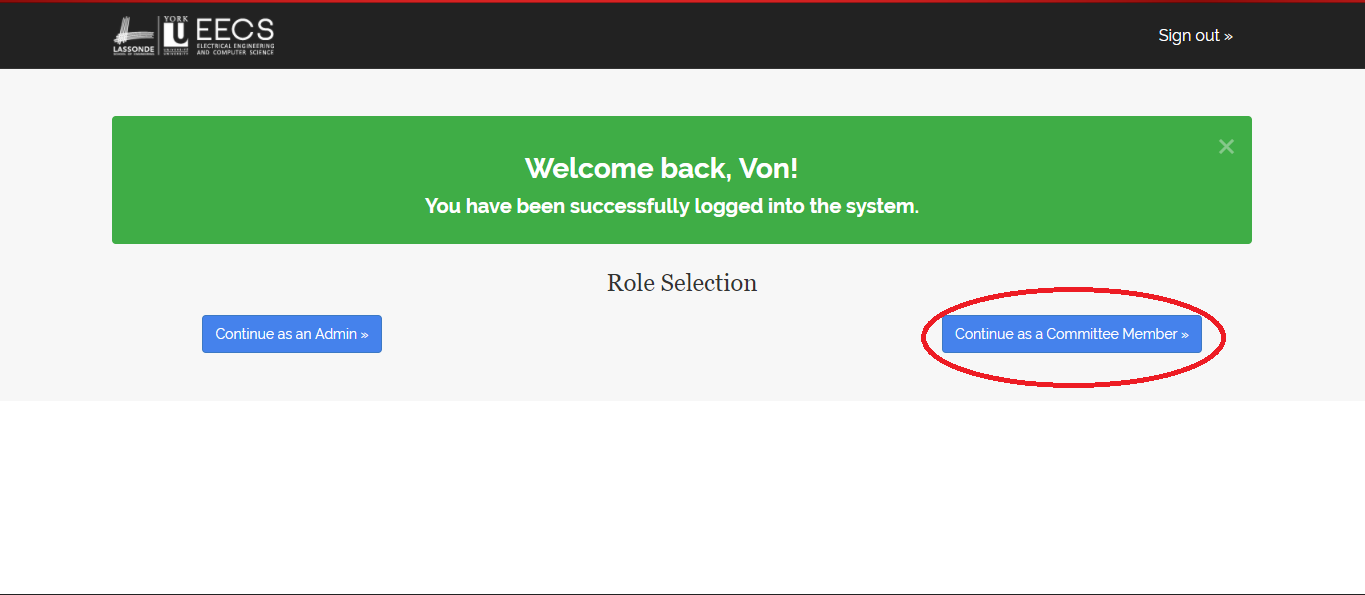
\includegraphics[width=.99\textwidth]{images/auth.png}
\end{center}
\caption{Role Selection Page}
\label{fig:role_selection1}
\end{figure}

\noindent \textbf{Note:} To access the administrator/committee/professor portal you must be granted access from an administrator.

\subsection{Navigation Bar}
If you have selected another role and wish to switch roles you will be presented with an option on the navigation bar. Click on the dropdown menu that displays your current role and click on your desired role.
\begin{figure}[!htb]
\begin{center}

\includegraphics[width=.99\textwidth]{images/role-selection2.png}
\end{center}
\caption{Switch Roles}
\label{fig:role_selection2}
\end{figure}

\noindent \textbf{Note:} To access the administrator/committee/professor portal you must be granted access from an administrator.

\clearpage

\section{Committee Member Portal}

After logging in and selecting the \emph{Committee Member} role you will have access to the committee member portal. In this portal you will be presented with a table containing all the students who have applied to be a graduate student. Here you can perform the following:
\begin{itemize}
\item View current and past reviewed application(s)
\item Apply filters on current and past reviewed application(s)
\item Review an assigned application(s)
\item Save a review as a draft for later completion.
\item Add new university assessments in the system to be used in a review. Such a new assessment will be added globally to the system and can be seen and used by other committee members when filling out a review.
\end{itemize} 

\begin{figure}[!htb]
\begin{center}
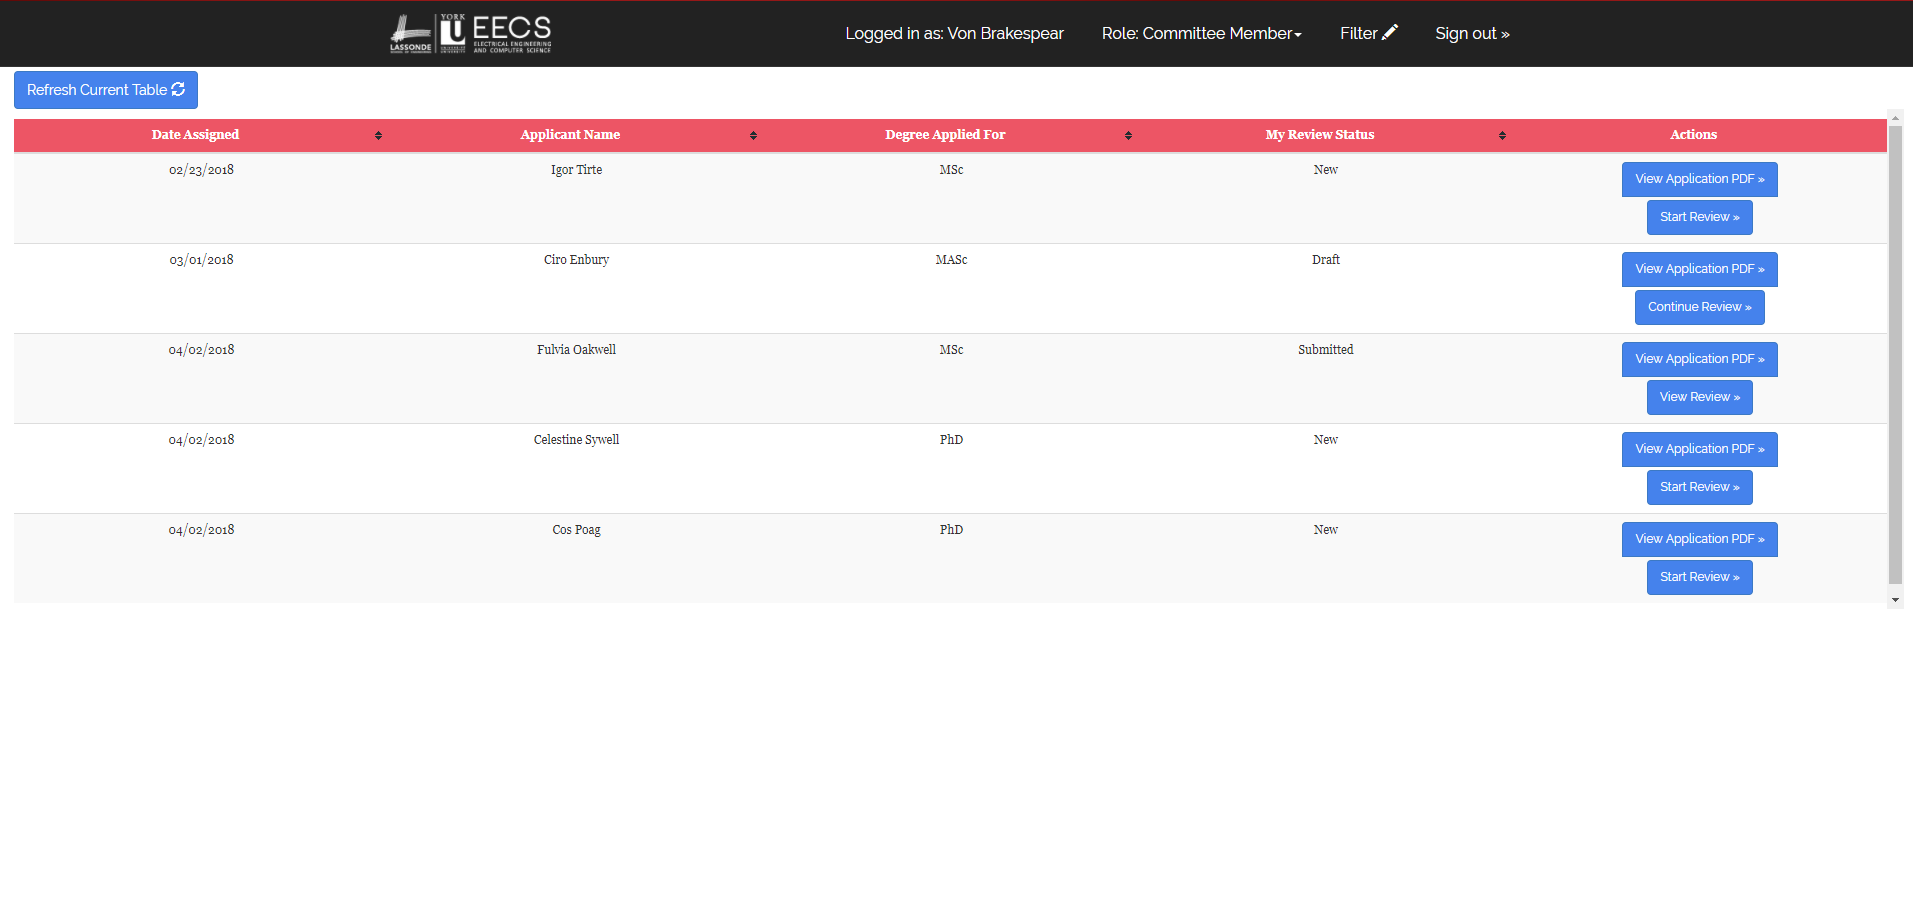
\includegraphics[width=.8\textwidth]{images/default_table.png}
\end{center}
\caption{Committee Member Portal}
\label{fig:cm_portal}
\textbf{Note:} If there are no reviews assigned, it will display a message instead. 
\end{figure}

\newpage
\subsection{Filtering the Table}
This section describes how you would use/build/save/load a filter on the table.
\begin{figure}[!htb]
\subsubsection{Opening the Modal}
To begin with filtering you must open the modal. To do so click on the ``Filter" button on the navigation bar.
\begin{center}
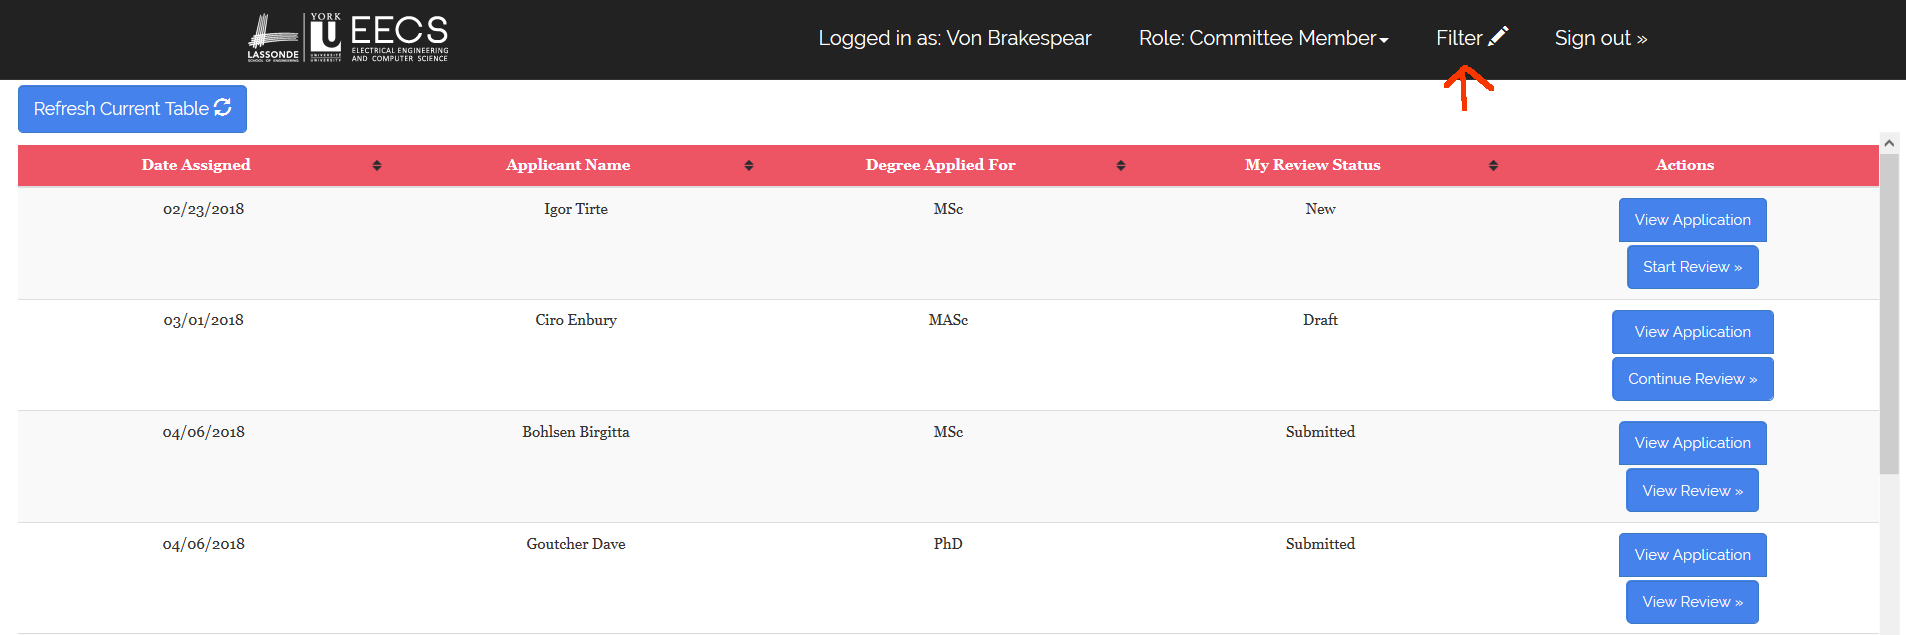
\includegraphics[width=.99\textwidth]{images/open_modal.png}
\end{center}
\caption{Opening the  Modal}
\label{fig:open_modal}
\end{figure}

\begin{figure}[!htb]
\begin{center}
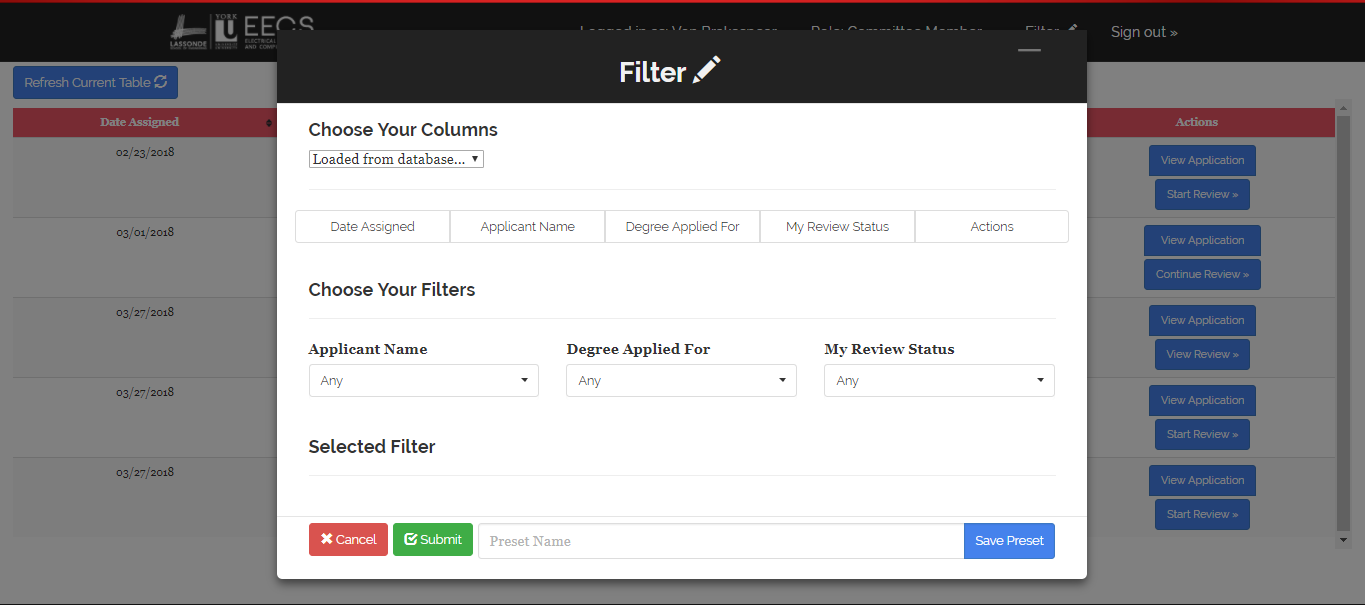
\includegraphics[width=.99\textwidth]{images/default_filter_view.png}
\end{center}
\caption{Filter View}
\label{fig:filter_view}
\end{figure}

\clearpage
\newpage

\begin{figure}[!htb]
\subsubsection{Choose Your Columns}
Once the modal is opened you can then choose the columns you wish to be displayed on the table. To do so, click on the button indicating which column you wish to see. Once clicked the button will display the order that column will appear in the table.\begin{center}
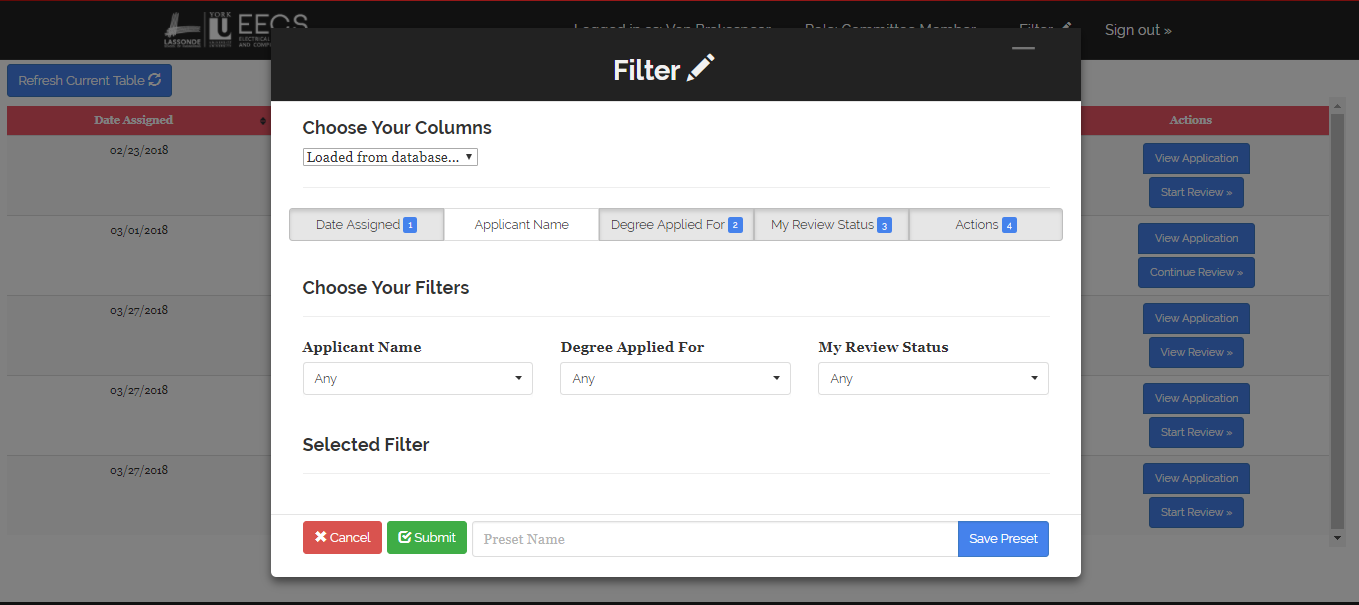
\includegraphics[width=.99\textwidth]{images/selected_col.png}
\end{center}
\caption{Choose Your Columns}
\label{fig:choose_columns}
\textbf{Note:} Not selecting any column will use the same columns and order as the default table. If the \emph{Actions} column is not selected it will automatically be placed as the right most column. 
\end{figure}

\clearpage
\begin{figure}[!htb]
\subsubsection{Choose Your Filters}
After selecting your columns, you can then choose the attributes by which you wish to filter your table. Begin by clicking on the drop down of the attribute you wish to filter and select an option from a list of generated options.
\begin{center}
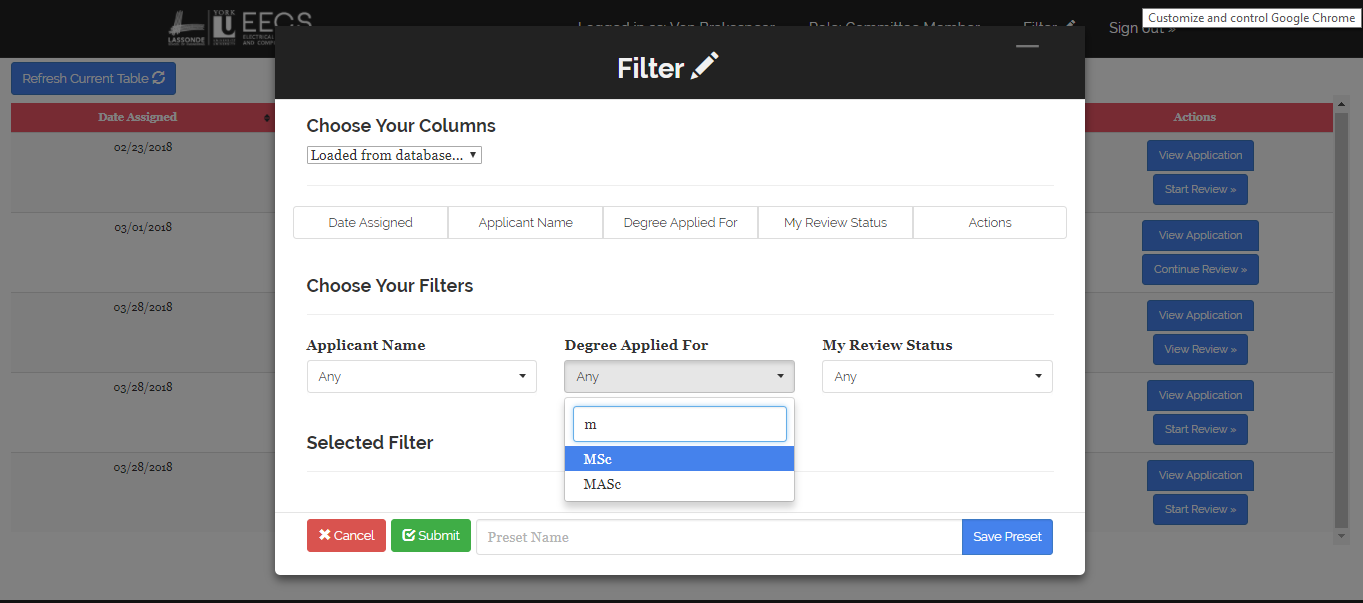
\includegraphics[width=.99\textwidth]{images/selected_filter.png}
\end{center}
\caption{Choose Your Filters}
\textbf{Note:} You can use the search bar to help locate values. Begin by typing in the text box displayed. You can only select an option that appears in the dropdown.
\label{fig:choose_filters}
\end{figure} 

\clearpage 
\begin{figure}[!htb]
\subsubsection{Submitting a Filter}
Once you have chosen your columns and filter attributes confirm your filter by reading the text under ``Selected Filter'' and click ``Submit". The text under the ``Selected Filter'' will change based on your filter attributes.
\begin{center}
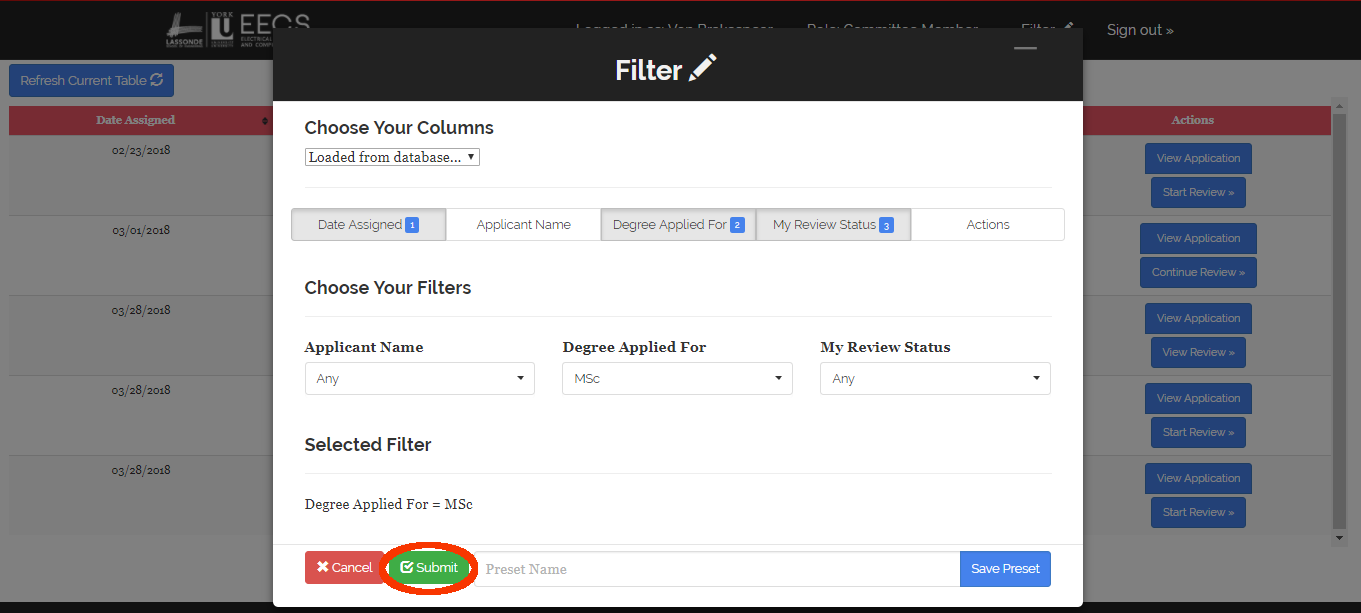
\includegraphics[width=.99\textwidth]{images/submit_filter.png}
\end{center}
\caption{Submit Filter}
\textbf{Note}: When submitting a filter with no selected filters, the default table will be loaded.
\label{fig:submit_filter}
\end{figure}

\begin{figure}[!htb]
\begin{center}
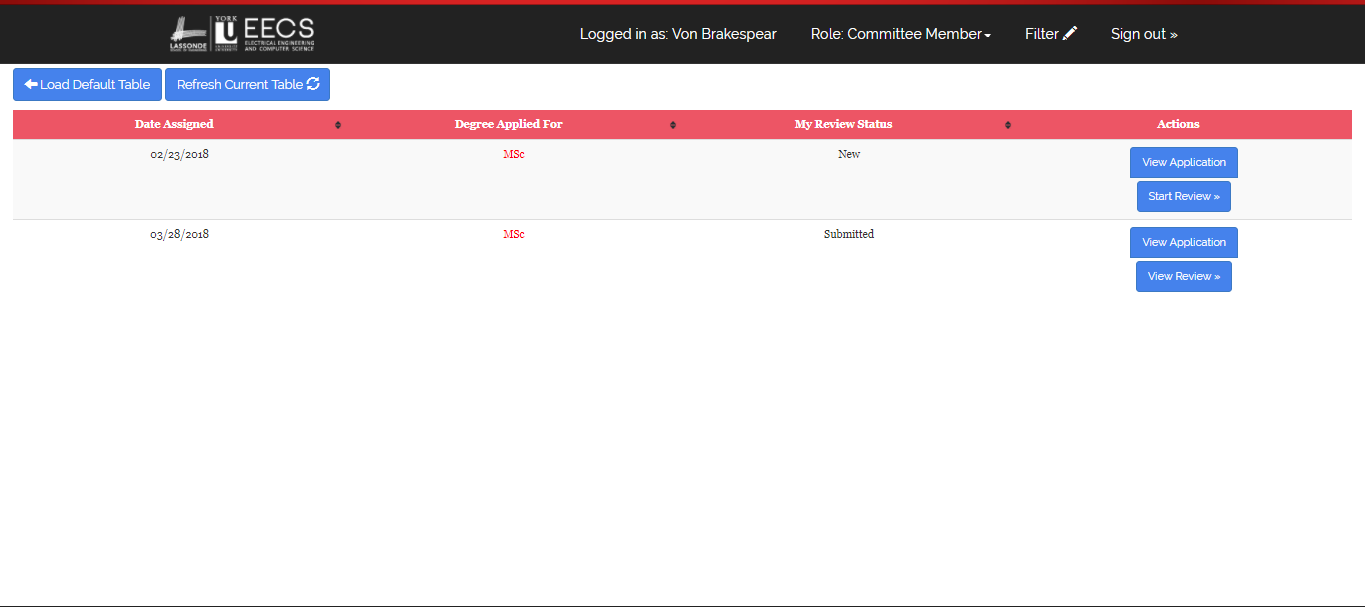
\includegraphics[width=.99\textwidth]{images/example_filter_table.png}
\end{center}
\caption{Resulted Table After Applying Filter}
\label{fig:resulted_table}
\end{figure}

\clearpage

\begin{figure}[!htb]
\subsubsection{Saving a Filter}
Once you have chosen your columns and filter attributes confirm your filter by reading the text under ``Selected Filter'' and give the preset a name by typing in the text box between the ``Submit'' and the ``Save Preset'' button. Once that is done click ``Save Preset''.
\begin{center}
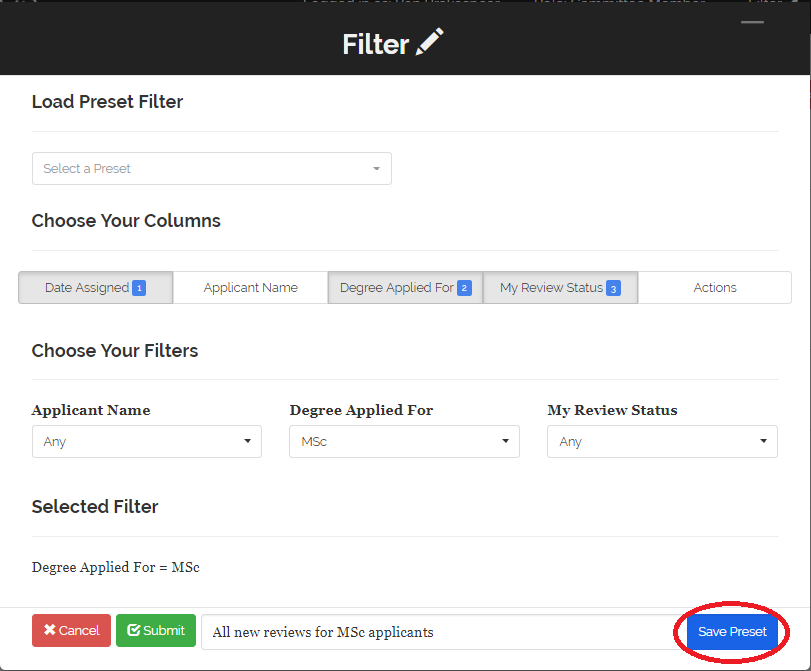
\includegraphics[width=.99\textwidth]{images/saving_preset.png}
\end{center}
\caption{Save a Filter}
Once you have saved a filter you will be provided with a new table to match your filter and it will appear in the dropdown to be used for loading a filter.\\
\textbf{Pro-tip:} You can update a filter by typing in the same name as an existing filter.
\label{fig:save_filter}
\end{figure}

\clearpage
\begin{figure}[!htb]
\subsubsection{Loading a Filter}
To load a saved filter click the dropdown under ``Load a Preset'' and select the preset you wish to use. Once selected the modal will auto-populate.
\begin{center}
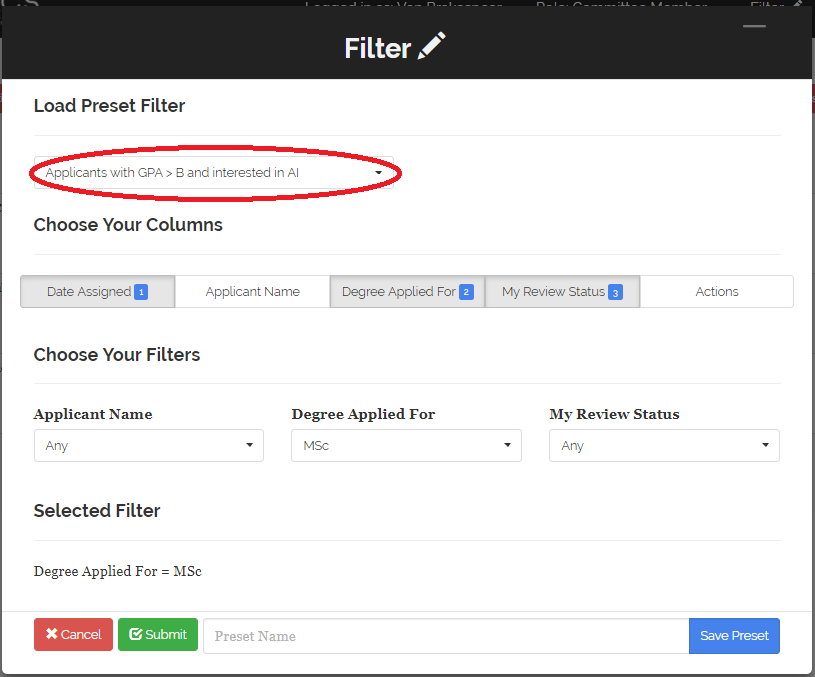
\includegraphics[width=.99\textwidth]{images/load_preset.png}
\end{center}
\caption{Loading a Filter}
\textbf{Pro-tip:} Create a preset called \emph{Default} with no columns or filters selected. You can then use this to load the default table or help clear any data you put in the modal.
\label{fig:save_filter}
\end{figure}
\clearpage
\newpage
\subsection{Sorting the Table}
If you wish to sort the table displayed simply click on the columns that display arrows next to the name. The table can be sorted in Ascending/Descending order described below.
\begin{itemize}
\item \textbf{Name:} Descending Order = Z to A, Ascending order = A to Z
\item \textbf{Date Assigned:} Descending Order = Newest - Oldest, Ascending order = Oldest - Newest
\item \textbf{Degree Applied For:} Descending Order = Z to A, Ascending order = A to Z
\item \textbf{Review Status:} Descending Order = Z to A, Ascending order = A to Z
\end{itemize}
\textbf{Pro-tip:} To sort by multiple columns hold the shift key while clicking on the columns.


\bigskip
\noindent \textbf{Note}: Ordering fields can be done on both filtered and unfiltered review application lists.

\bigskip
\noindent The following images depicts on how to order review applications using the \emph{Date Assigned} field in ascending and descending order.

\begin{figure}[!htb]
\begin{center}
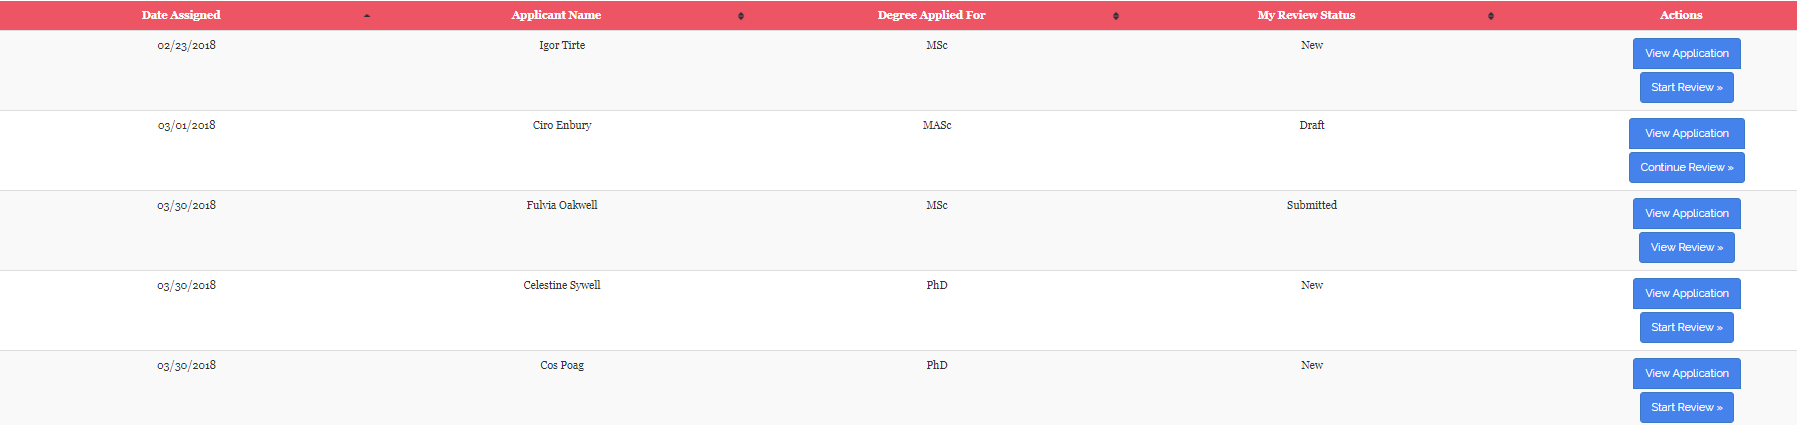
\includegraphics[width=.99\textwidth]{images/order_ascending.png}
\end{center}
\caption{Ascending order of Date Assigned field}
\label{fig:order_ascending}
\end{figure}

\begin{figure}[!htb]
\begin{center}
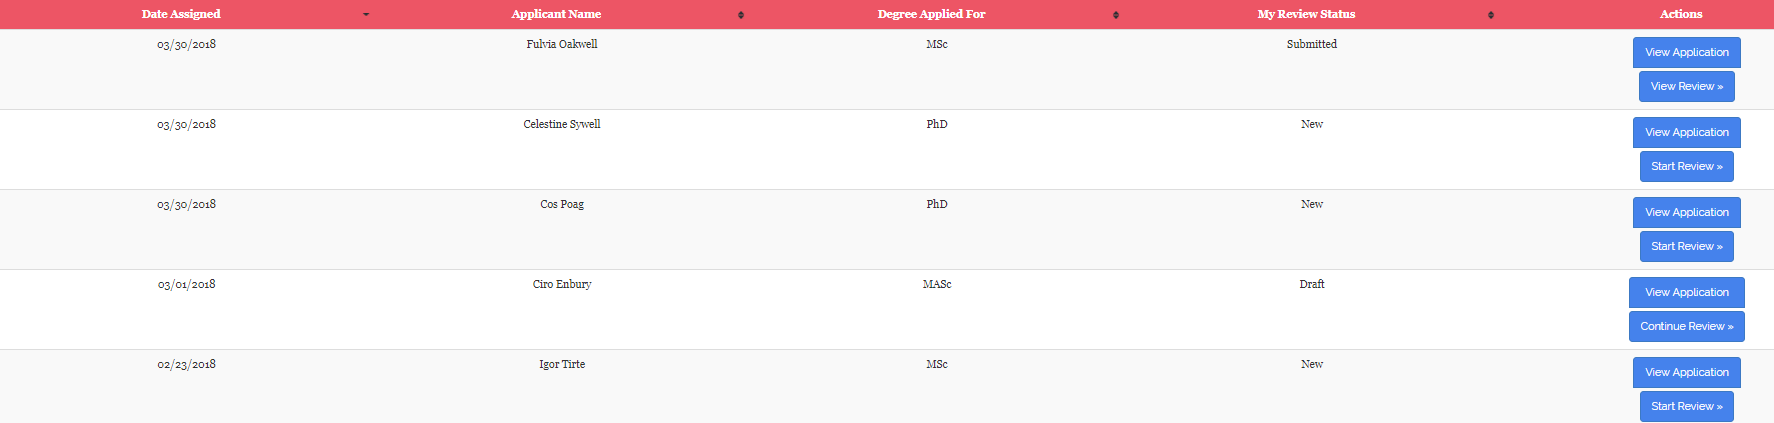
\includegraphics[width=.99\textwidth]{images/order_descending.png}
\end{center}
\caption{Descending order of Date Assigned field}
\label{fig:order_descending}
\end{figure}

\newpage

\begin{figure}[!htb]
\begin{center}
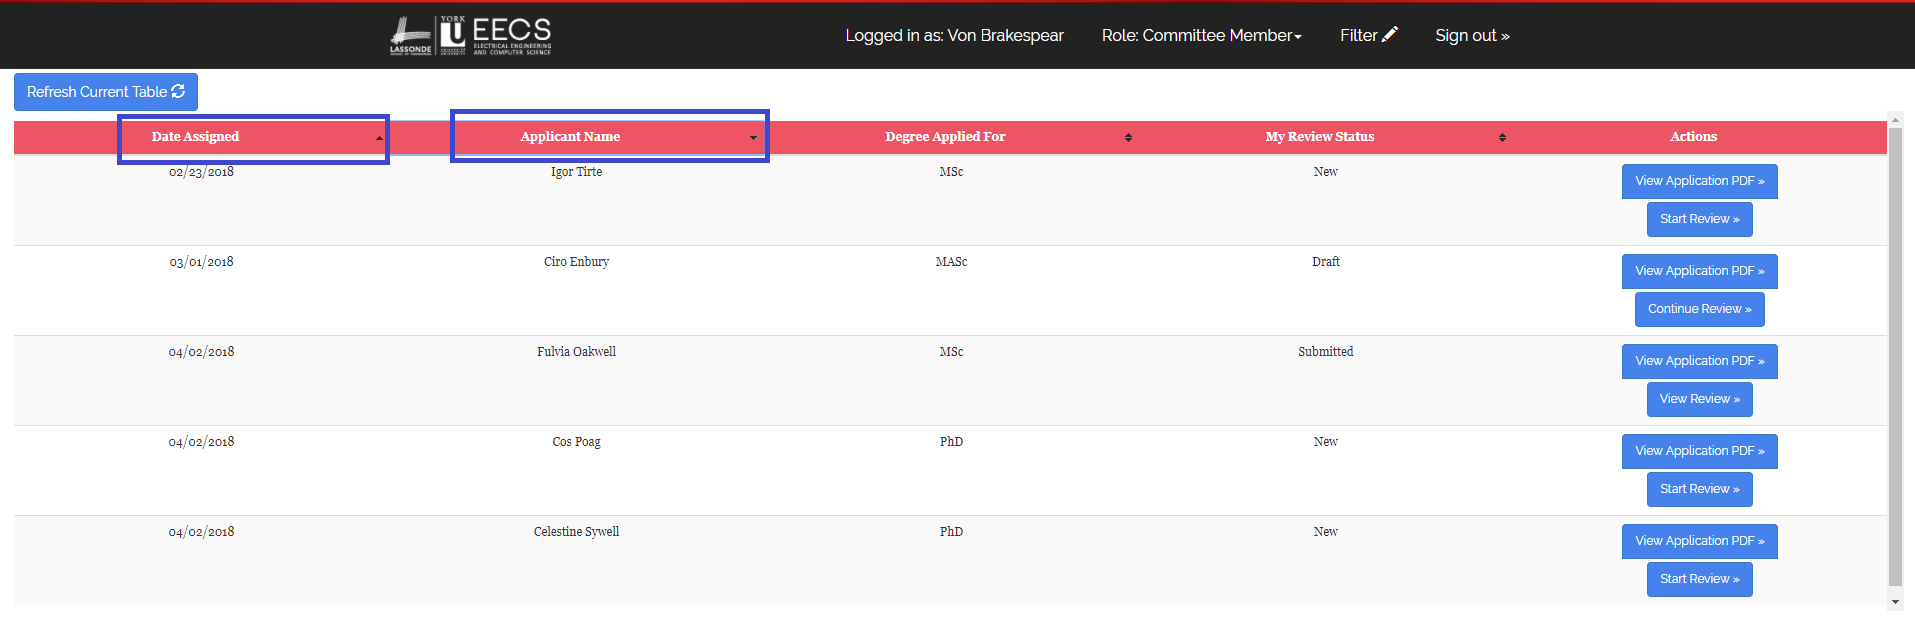
\includegraphics[width=.99\textwidth]{images/multiple_order.png}
\end{center}
\caption{Ordering using multiple fields}
\label{fig:multiple_order}
\end{figure}

\clearpage
\newpage
\section{Reviewing Applications} \label{sec:reviews}
The review process can have \textbf{three} different statuses shown
\begin{itemize}
\item \textbf{New}: A new application has been assigned to the committee member and no changes have been made on the review yet.
\item \textbf{Draft}: A previously saved draft review. A review is considered as a draft when there has been at least one or more changes committed and the user has decided to save the changes.
\item \textbf{Submitted}: A completed review which has been submitted and uploaded to the server. Once a review is submitted, it cannot be undone.
\end{itemize}

\bigskip
\noindent The following list denotes the fields in a review form that is \textbf{not} submitted yet and their requirement status:
\begin{table}[h]
\centering
\begin{tabular}{|c | c |}
	\cline{1-2}
	\textbf{Field Name} & \textbf{Required}\\ \hline
	Institution Name(s) & No \\ \hline
	Institution Assessment(s) & No \\ \hline
	Background Information & No \\ \hline
	Research Experience & No \\ \hline
	Letter of Intent Analysis & No \\ \hline
	Additional Comments & No \\ \hline
	Applicant Rank & Yes \\ \hline
\end{tabular}
\caption {Review Fields}
\label{tbl:review_fields}
\end{table}

\newpage
\bigskip
\noindent The following image depicts the full view of the review form. The \emph{View Application PDF} link opens the student application in PDF version uploaded by the system administrator. 

\begin{figure}[!htb]
\begin{center}
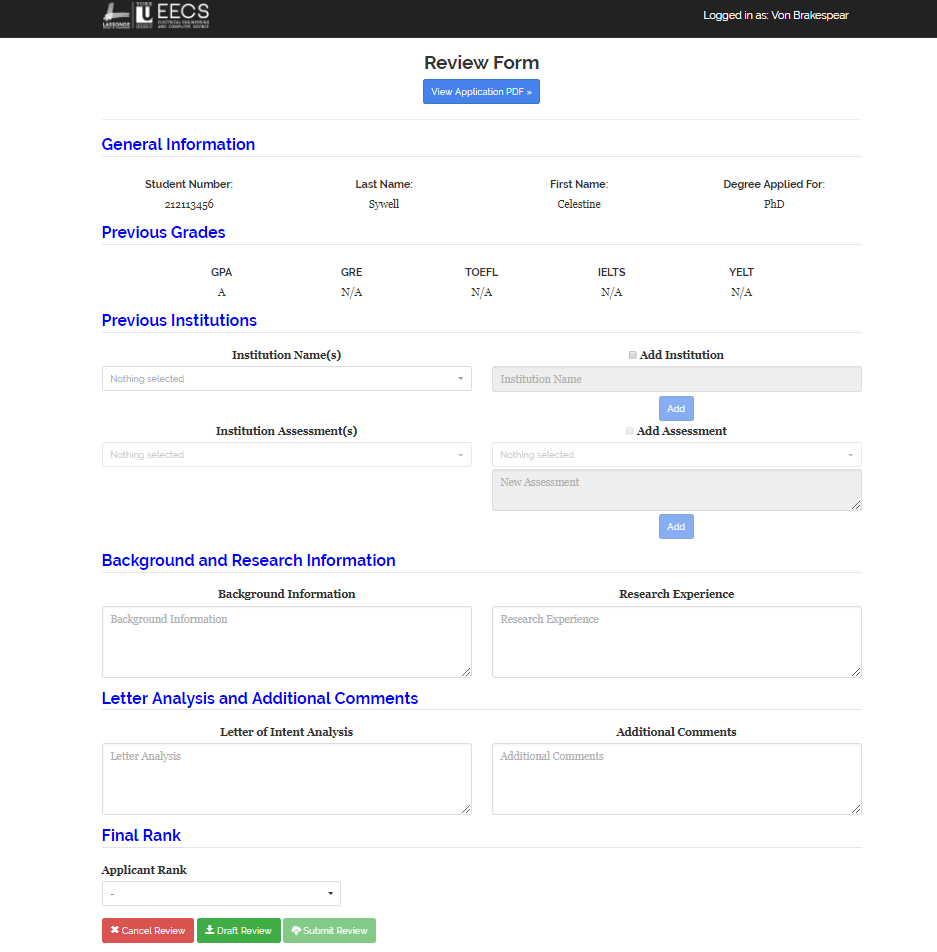
\includegraphics[width=.99\textwidth]{images/review_form.png}
\end{center}
\caption{Full view of the Review Form}
\label{fig:review_form}
\end{figure}

\clearpage
\newpage
\subsection{Opening a new Review}
When a new review is received it will show on the portal. After that you will have the option of opening the review and start completing the form. The action for opening a new review will say \textbf{Start Review}.

\bigskip
\noindent The following image depicts user opening a brand new review.

\begin{figure}[!htb]
\begin{center}
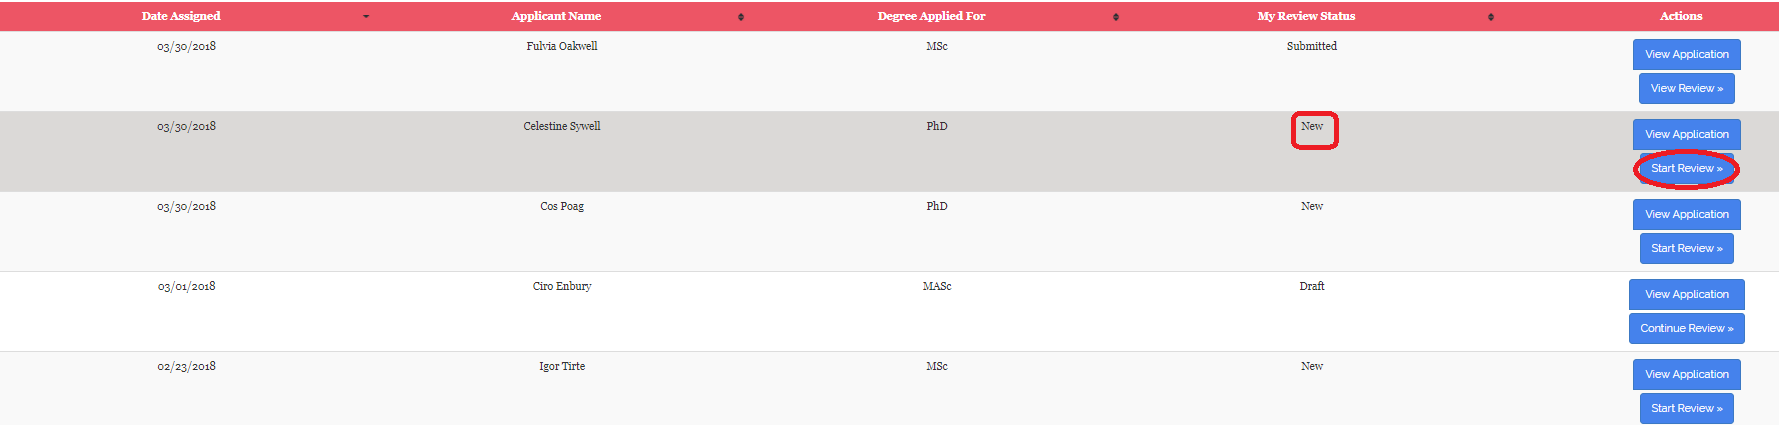
\includegraphics[width=.99\textwidth]{images/opening_new_review.png}
\end{center}
\caption{Opening a brand new review}
\label{fig:opening_new_review}
\end{figure}

\bigskip
\noindent The following image depicts user making no changes to the opened review and exiting out of the review form.

\begin{figure}[!htb]
\begin{center}
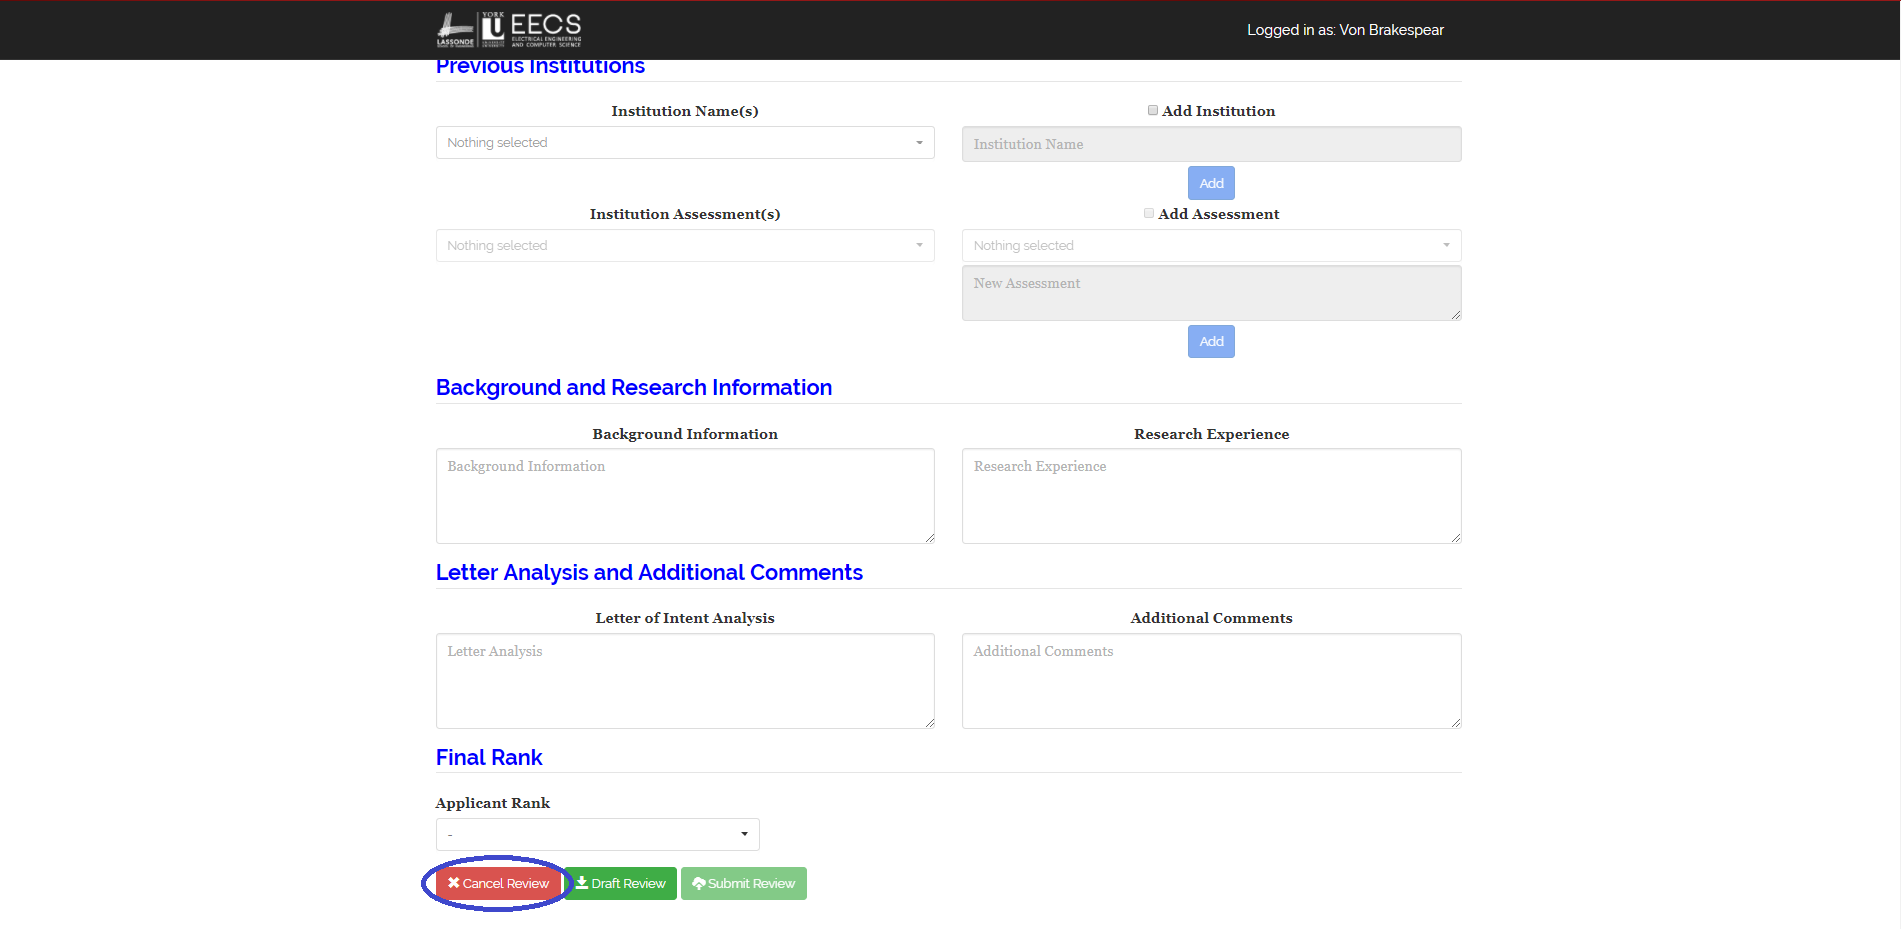
\includegraphics[width=.99\textwidth]{images/new_review_exit_wo_changes.png}
\end{center}
\caption{Exiting out of a brand new review application without changes}
\label{fig:new_review_exit_w/o_changes}
\end{figure}

\subsection{Filling out a Review}
Table \ref{tbl:review_fields} outlines the fields in a review application and their required status. The following table specializes Table \ref{tbl:review_fields} and displays the type of input each field takes.

\begin{table}[h]
\centering
\begin{tabular}{|c | c |}
	\cline{1-2}
	\textbf{Field Name} & \textbf{Input Type}\\ \hline
	Institution Name(s) & Multiple Drop-Down \\ \hline
	Institution Assessment(s) & Multiple Drop-Down \\ \hline
	Background Information & Text \\ \hline
	Research Experience & Text \\ \hline
	Letter of Intent Analysis & Text \\ \hline
	Additional Comments & Text \\ \hline
	Applicant Rank & Single Drop-Down \\ \hline
\end{tabular}
\caption {Review Fields Input Type}
\label{tbl:review_fields_input}
\end{table}

\subsubsection{Institution Assessment}
When performing a institution assessment you can select from one or more institutions and a description in the database. If the institution does not exist or their description is inadequate you can also create a new institution/assessment.

\bigskip
\noindent The following image depicts an user selecting two institutions the applicant has attended and selecting an assessment from each of the institutions.

\begin{figure}[!htb]
\begin{center}
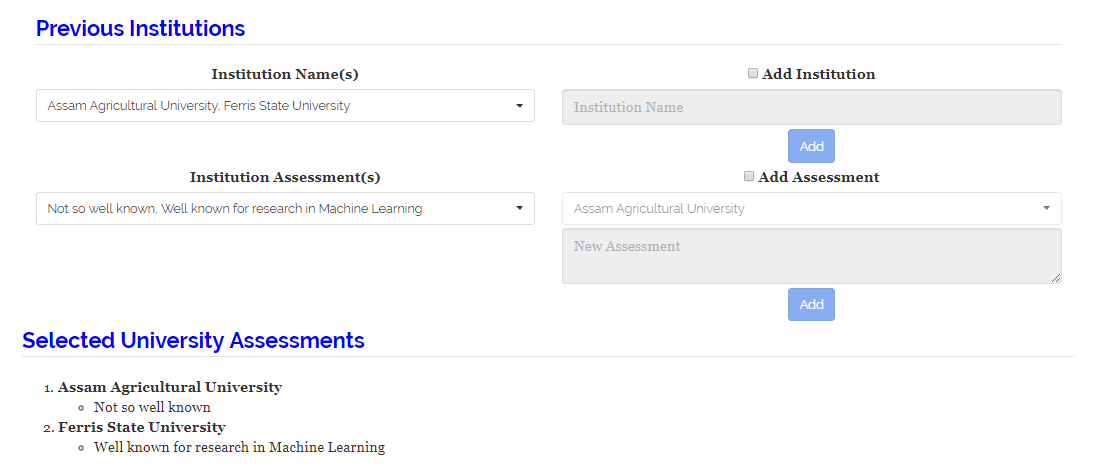
\includegraphics[width=.7\textwidth]{images/uni_assessment.png}
\end{center}
\caption{Institution Assessment View}
\label{fig:uni_assessment}
\end{figure}

\clearpage
\newpage
\subsection{Saving a Review as Draft}
While filling out a review you will have the opportunity to save an on-going review as a draft for future completion.

\bigskip
\noindent The following images depicts a user making changes to an application review and then saving it as a draft. Consequently, the status of the review is changed to \textbf{Draft}. And if the user wants to continue working on the draft sometime later, the action for opening a drafted review will say \textbf{Continue Review}.

\begin{figure}[!htb]
\begin{center}
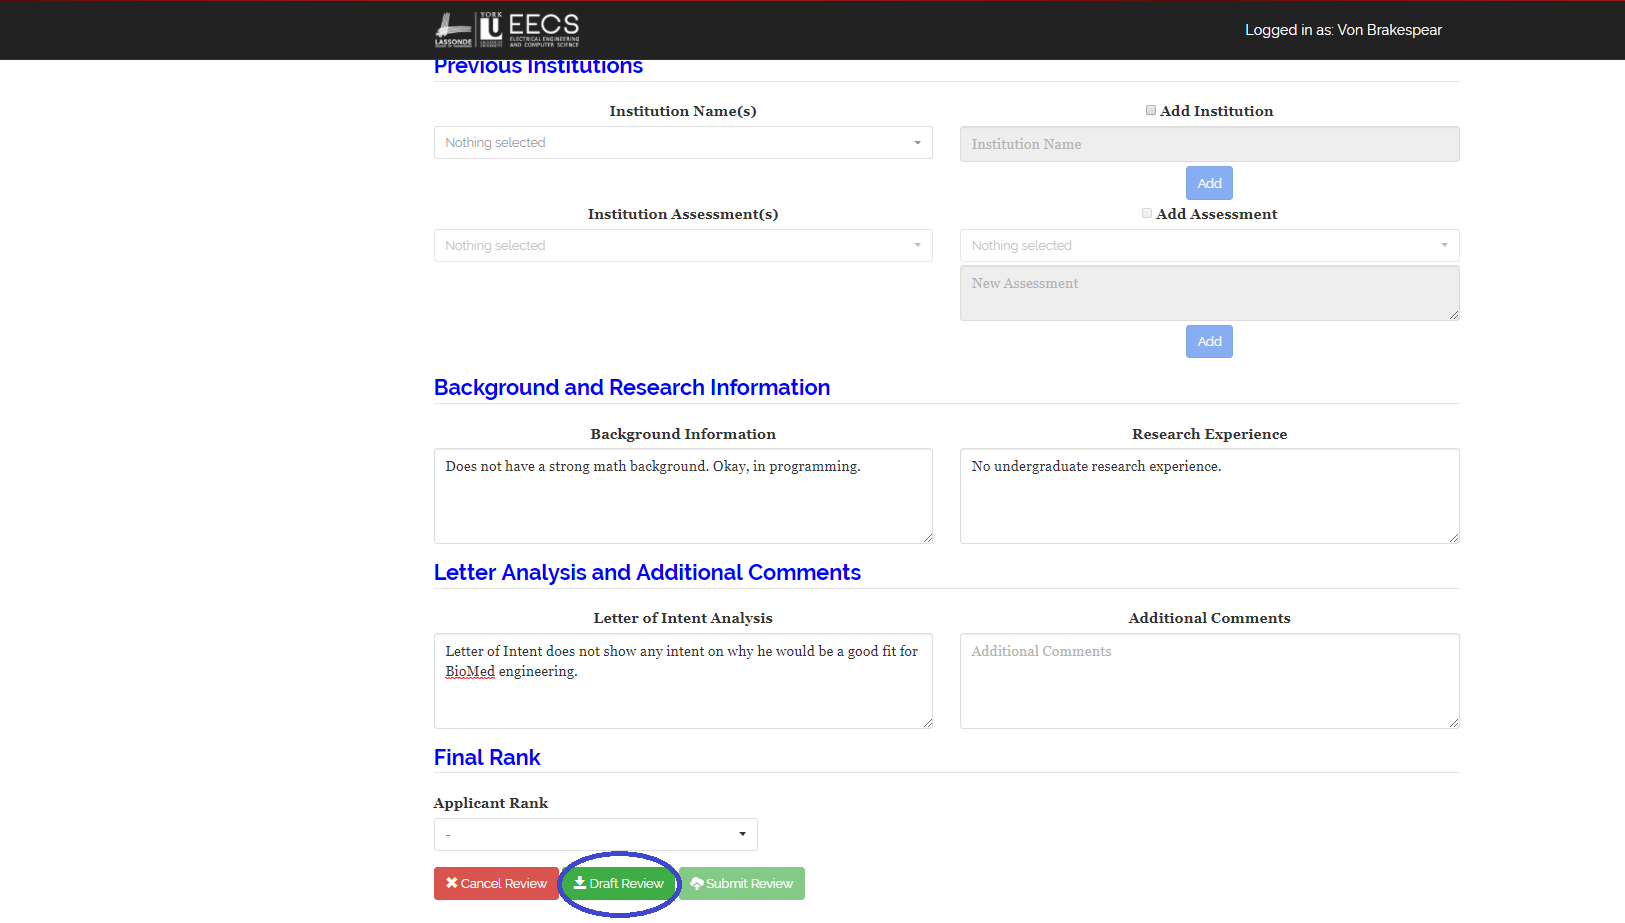
\includegraphics[width=.99\textwidth]{images/save_as_draft_review.png}
\end{center}
\caption{Save a review as draft}
\label{fig:save_as_draft_review}
\end{figure}

\begin{figure}[!htb]
\begin{center}
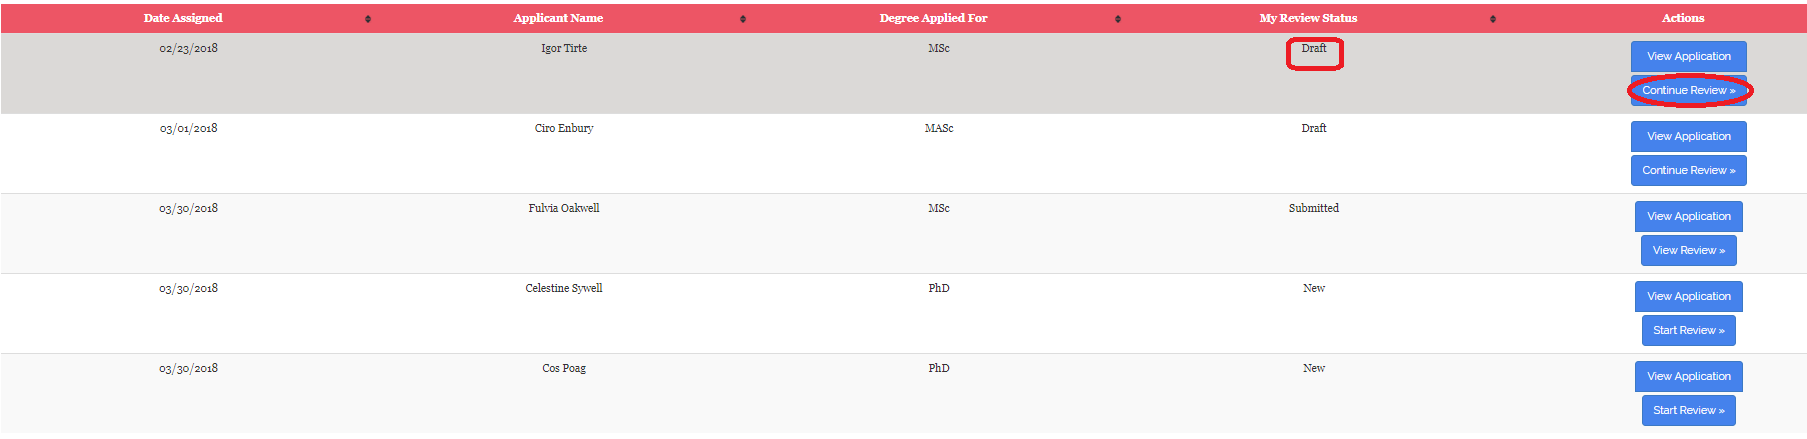
\includegraphics[width=.99\textwidth]{images/drafted_review.png}
\end{center}
\caption{Drafted Review View}
\label{fig:drafted_review}
\end{figure}

\subsection{Submitting a Review}
Once you are satisfied with your review simply  click the \textbf{Submit Review} button to complete your review. If the correct number of reviews for an application has been submitted (depending on visa status), the application will be automatically available for selection to those on the \textbf{Professor Portal}. The only required field needed for submitting a review is the final application rank that is to be decided by the admission committee member upon analysing the application.

\bigskip
\noindent The following image depicts an end user submitting a review. 

\begin{figure}[!htb]
\begin{center}
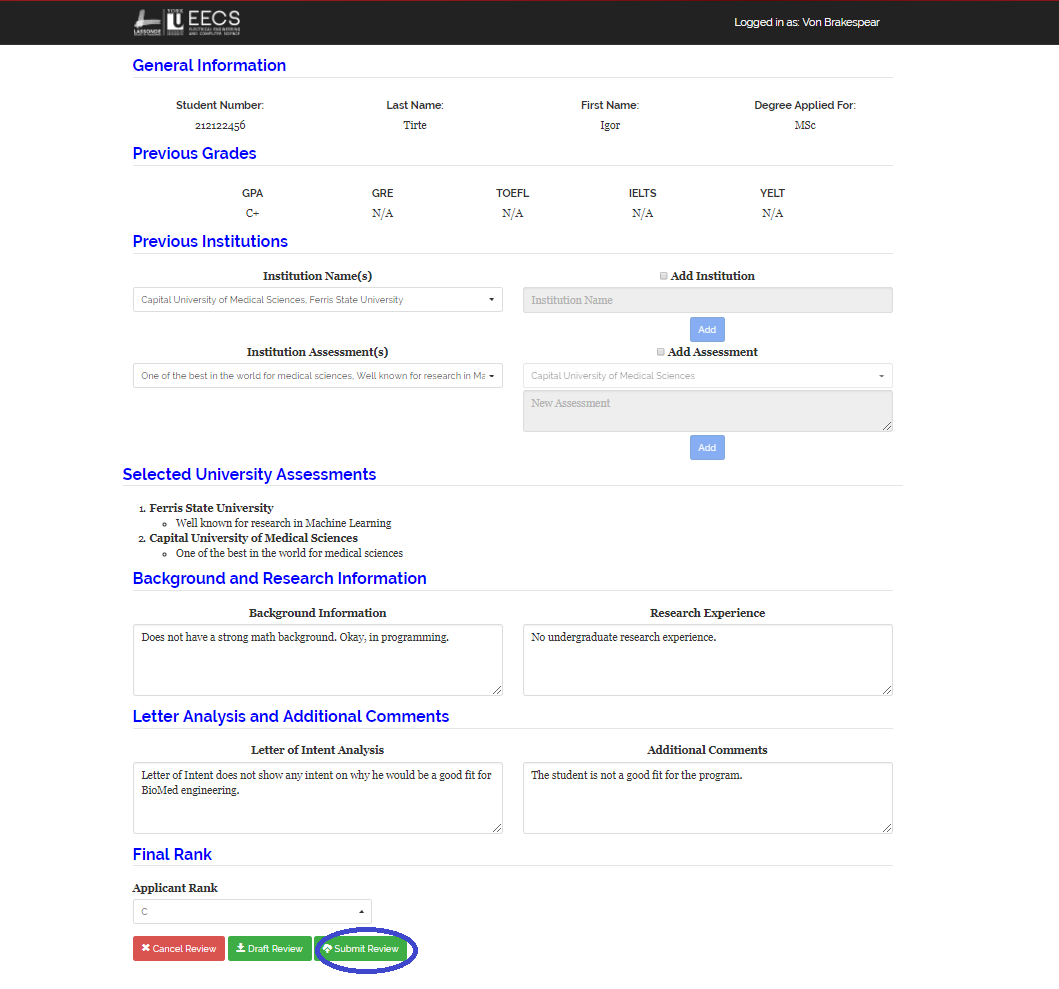
\includegraphics[width=.99\textwidth]{images/submit_review.png}
\end{center}
\caption{Submit a Review}
\label{fig:submit_review}
\end{figure}
\clearpage
\bigskip
\noindent Once the review is submitted, it will show up on the user dashboard with status as \textbf{Submitted} and The user action to view a submitted review will say \textbf{View Review}. Submitted reviews are only viewable as a plain text application form. The following images depicts viewing a submitted review.

\begin{figure}[!htb]
\begin{center}
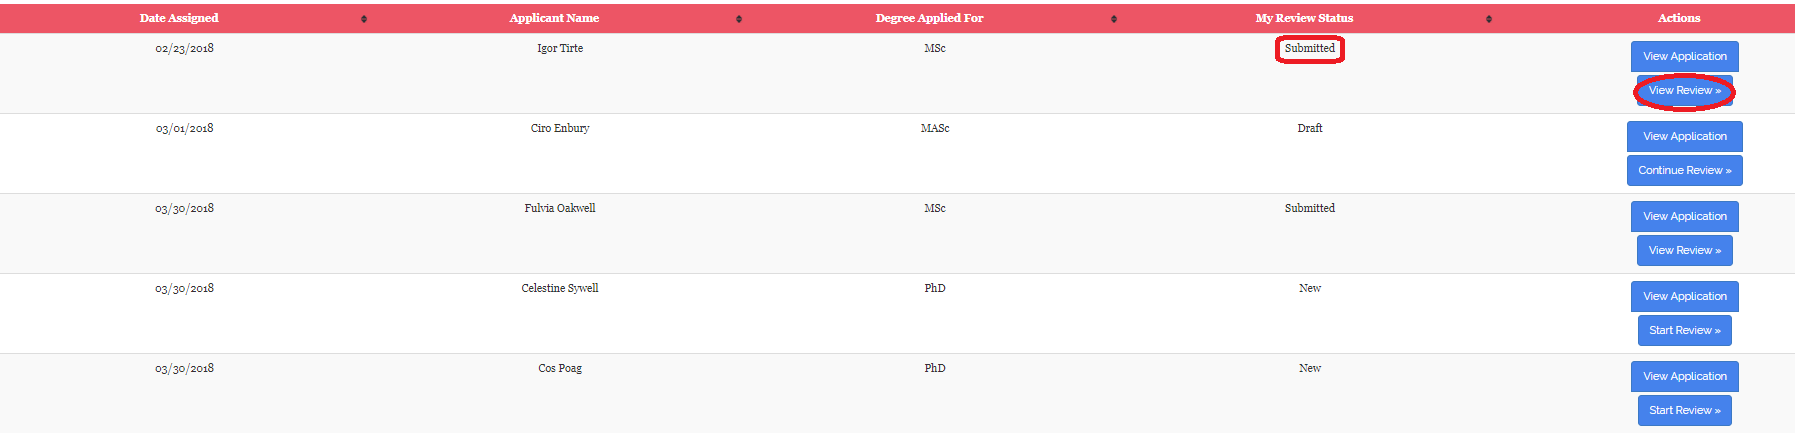
\includegraphics[width=.99\textwidth]{images/submitted_review.png}
\end{center}
\caption{Submitted Review View}
\label{fig:submitted_review}
\end{figure}

\begin{figure}[!htb]
\begin{center}
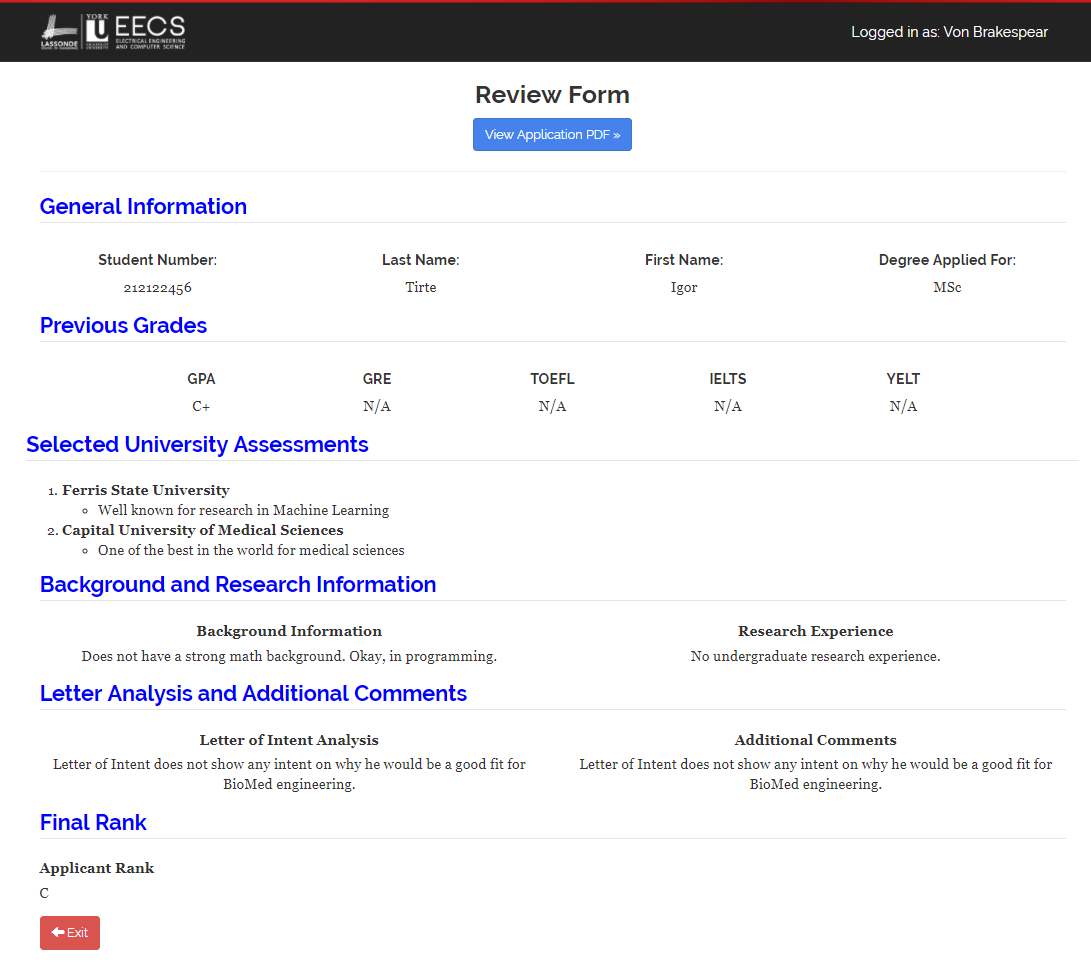
\includegraphics[width=.99\textwidth]{images/submit_review_view.png}
\end{center}
\caption{Submitted Review View}
\label{fig:submit_review_view}
\end{figure}

\end{document}